%================================================================================
%== SETUP - CAN IGNORE
%================================================================================

%below is where we can change font of slides
\documentclass[9pt,letterpaper,subeqn]{beamer}
\setbeamertemplate{navigation symbols}{}
\setbeamertemplate{footline}{\begin{center}\small\insertframenumber\end{center}}
\usefonttheme{serif}
\usecolortheme{orchid}



\usepackage[english]{babel}
\selectlanguage{english}
\usepackage{bm}
\usepackage{booktabs}
\usepackage{color}
\usepackage[update,prepend]{epstopdf}
\usepackage{framed}
\usepackage{fleqn}
\usepackage{graphics}
\usepackage{hyperref}
\usepackage[utf8]{inputenc}
\usepackage{setspace}
\usepackage{textcomp}
\usepackage{wrapfig}
\usepackage{multirow}
\usepackage{caption}
\usepackage{subcaption}
\setbeamertemplate{caption}[numbered]

%================================================================================
%== TITLE, NAMES, DATE
%================================================================================
\title{The Twin Instrument and The Fertility-Investment Trade-off}
%make his into normal author tex symbol
\author{Sonia Bhalotra\inst{\dag} \and Damian Clarke\inst{\ddag}}
\institute{\inst{\dag} University of Essex \and \inst{\ddag} University of Oxford & University of Santiago}
\date{May 2016}



\begin{document}


\begin{frame}
\titlepage
\end{frame}


%%Damian i started before you woke up and so i started on the tex file used for the Germany/Essen talk in Apr-2015. Looking at the PDF of this i think it is worth experimenting with using a slightly 
%smaller font so we get less crowded slides, with more spaces
%%RESPONSE: No problem.  I will do this once I compile the first time.  Above where it says "10pt" (after documentclass) we can change it to 9pt.

%While editing in tex i am not sure how crowded my slides are so after the first compilation we can break some into 2 parts.
%%RESPONSE: Yes, makes sense!  Feel free to write and then once compiling we can shift around based on how it looks.

%================================================================================
%== Twins: A Natural Experiment
%================================================================================

\section{Introduction}

\frame{\frametitle{Twins As A Natural Experiment}
\begin{itemize}
\item A vast literature in economics, behavioural genetics and psychology relies upon the premise that twin births occur as an act of nature -- and are allocated randomly across families.\\ \vspace{5mm}
\item A twin birth generates a natural experiment. 
\begin{itemize}
\item It allows us to compare families that unexpectedly have an additional child because they have a twin birth with families who have the same number of birth events but only singleton births. \\ \vspace{5mm}
\end {itemize} 
\item This is useful when one is interested in identifying causal effects of fertility (number of children) on investments in child quality (e.g. education), or on mothers' workforce participation.
\end{itemize}
}



%================================================================================
%== Twin Births Are Not Random
%================================================================================


\frame{\frametitle{Our Critique: Twin Births Are Not Random}
\begin{itemize}
\item Even if twin conceptions are `random', twin births are not because taking twins to term depends on health stocks and behaviours of mothers during pregnancy.
\item If health and health-seeking behaviour are correlated with the outcomes, the natural experiment breaks down.\\ \vspace{5mm}
\item We present the first evidence that this is a widespread phenomenon in rich and poor countries
\item In poor countries, many women are severely under-nourished and may not be fit enough to carry twin conceptions to birth, and antenatal services are weak. 
\item In richer countries, many women engage in risky behaviours and/or experience medical problems in pregnancy.
\end{itemize}
}

%================================================================================
%== Mechanism
%================================================================================


\begin{frame}[label=mech]
\frametitle{Mechanisms}
\item The mechanism we propose is selective foetal death. 
	\begin{itemize}
	\item Twin conceptions are more demanding of maternal resources \& hence more likely to suffer miscarriage or stillbirth.
	\item About 1 in 8 twin conceptions results in a live birth. Spontaneous abortion rate among twins three times that for singletons (Boklage 1990). \\ \vspace{3mm}
	\item Supporting medical evidence: FSH is associated with the risk of dizygotic twins and is more prevalent among heavier and taller women (Li et al.\ 2003, Hall 2003) \\ \vspace{3mm}
	\end{itemize}
\item We  provide evidence in favour of this mechanism.
\end{itemize}
\end{frame}
}

%================================================================================
%== Invalidity of Twin IV
%================================================================================


\frame{\frametitle{Maternal Health- Multidimensional, Unobservable}
\begin{itemize}
\item Maternal health and pregnancy behaviours are multidimensional and at best partially observed.
\item Therefore impossible to adjust for them and restore validity of the twin instrument.
\item Examples of unobservables include stress, sleep, breakfast-skipping, folic acid supplementation, pollution exposure.
\end{itemize}
}


%================================================================================
%== Why Do We Care
%================================================================================

\frame{\frametitle{Relevance of this Critique}
\begin{itemize}
\item Estimates using twins to instrument fertility are biased on account of mothers of twins being positively selected.
\item Plausible that women's health is positively correlated with their labour supply and the quality of their children.
\item If so, the twin-IV estimator will tend to under-estimate the tradeoffs between fertility and (a) labour supply and (b) child quality.
\item Relevant to lively scholarly and policy interest in the career costs of children (Adda et al. 2015) and the quantity-quality tradeoff (Angrist et al. 2010).  
\item Relevant for instance to motivating fertility-control policies (China vs Italy).
\end{itemize}
}


%================================================================================
%== The Quantity-Quality Tradeoff
%================================================================================

\frame{\frametitle{The Quantity--Quality Trade-off}
\begin{itemize}
\item In this paper, to illustrate the problem, we focus upon the QQ tradeoff.
\item Empirical regularity- cross-section & time series- large families are associated with weaker educational outcomes (Hanushek 1992, Blake 1989, Galor 2012). \vspace{3mm}
\item Could signify a QQ trade-off (Becker and Lewis 1973, Becker and Tomes 1976) or, alternatively, shift factors like income. \vspace{3mm}
\item Recent studies using the twin instrument reject the Q-Q tradeoff (Angrist et al.\ 2010, Black et al.\ 2005), while other approaches do not (Cohen et al. 2013).
\item We argue that an underlying trade-off is veiled by the IV-bias created by omitted maternal health. 
\end{itemize}
}


%================================================================================
%== What We Do
%================================================================================

\frame{\frametitle{What We Do}
\begin{itemize}
\item Demonstrate that twin births are correlated with maternal health using cross-sectional and within-mother variation in microdata from many countries.
\item Provide evidence of the driving mechanism i.e. that twin births are more likely to miscarry, and especially among less healthy women.
 
\item Present OLS estimates: Potential negative selection of women into high fertility.
\item Present IV estimates: Potential positive selection of women into high fertility.
\item True estimate will lie between the OLS and IV estimates.
\end{itemize}
}

\frame{\frametitle{What We Do- continued}
\begin{itemize}
\item First-stage IV: Show that twins are a powerful predictor of fertility.
\item Second-stage IV: Show (partial) bias-correction following (partial) adjustment for maternal health and other characteristics.
\item Adjustment for maternal characteristics will narrow the gap [bounds] between the OLS and IV estimates.
\end{itemize}

\item Estimate bounds on the IV estimates on premise that twins are plausibly (rather than strictly) exogenous (Conley et al. 2012).
\item Provide estimates for the USA and for a pooled sample of developing countries.
\end{itemize}
}


%================================================================================
%== Data
%================================================================================

\section{Data}
\frame{\frametitle{Data}
\begin{itemize}
\item Large samples are useful given twins are rare (around 2\%) 
\item This said, twins are not as rare as we may think: 1 in 80 livebirths, so 1 in 40 babies is a twin.
\item Comparable cross-country micro-data for developing countries
\item Surveys conducted 1991-2013: sample of ~3m. children born in 68 countries. Birth cohorts 1971-2012 (condition on country and birth cohort FE)\\ \vspace{5mm}
\item American National Health Interview Surveys conducted 1997-2013 \\ \vspace{5mm}
\item Administrative birth registries and surveys from the UK, Scotland, Sweden, Chile, Spain.
\end{itemize}
}

%%% Damian can we create a new slide here which is just a title slide that says Part I: Showing that twins are more likely to be born of healthy mothers. Then we will have similar title slides for 
%% Parts 2 and 3 of the paper below
%%RESPONSE: The below slide will do this.  I can add in others v easily.
\frame{
\begin{center}
\Large Showing that twins are more likely to be born of healthy mothers
\end{center}
}

%================================================================================
%== Part I: Showing Twin births are not random- CS
%================================================================================

\frame{\frametitle{Twins have selectively healthy mothers- CS}

\begin{enumerate}
\item Cross-sectional microdata evidence from many rich and poor countries.
\item Regress twin birth on indicators of maternal health, $\bm{H}$ (height, BMI during pregnancy, antenatal care availability, smoking/drinking/drugs and medical problems during pregnancy  
\item Conditional upon $\bm{X}$ (age, parity, race, ethnicity) and $\bm{S}$ (wealth, education). \vspace{3mm}
\end{enumerate}

\begin{equation}
\label{TWINeqn:twinreg}
P(twin_{j})=\gamma_0 + \bm{X}\bm{\gamma}_1 + \bm{S}\bm{\gamma}_2
                  + \bm{H}\bm{\gamma}_3 + \varepsilon_{j}.
\end{equation}

\begin{itemize}
\item If twin birth is a random event $\bm{\gamma_1}=\bm{\gamma_2}=\bm{\gamma_3}=0$.
\item Except for maternal age and parity which are factors that geneticists have previously associated with twin births. 
\item Equivalent to a test for balance of characteristics of `treated' (with twins) and `control' (without twins) mothers.
\item Confirm that the association of interest holds for cohorts born prior to the introduction of IVF.
\end{itemize}

}



%================================================================================
%== Showing Twin births are not random- within mother
%================================================================================
\frame{\frametitle{Twin births are more likely in health families: within mother}
\vspace{5mm}

\begin{itemize}
\item Within-mother microdata evidence from poor countries. 
\item Consider families with at least two births. 
\item Compare infant mortality of first births followed by a twin with that of first births followed by a singleton. 
%\item Hypothesis is that first-born children are healthier in families that subsequently have twins. \vspace{3mm}
\end{itemize}

\vspace{2mm}
\[Infant health_{t-k}=\alpha twins_{t}+\bm{X}\delta + \varepsilon \]
\vspace{5mm}

\begin{itemize}
\item If twins occur randomly, $\alpha=0$.  If positively selected, $\alpha<0$.
\item Can think of infant mortality as an index of maternal health. 
\item In this case, also useful to think of it as an indicator of child quality.
\end{itemize}

\end{itemize}
}

%================================================================================
%== Results- within mother- 
%================================================================================

\frame{\frametitle{Are healthy mothers more likely to produce twins?}
\begin{table}[htpb!]\caption{IMR Test} 
\label{TWINtab:IMR}\vspace{-5mm}\begin{center}\begin{tabular}{lccc}
\toprule \toprule 
\textsc{IMR}& Base & +S\&H & Observations \\ \midrule 
\begin{footnotesize}\end{footnotesize}& 
\begin{footnotesize}\end{footnotesize}& 
\begin{footnotesize}\end{footnotesize}& 
\begin{footnotesize}\end{footnotesize}\\ 
Treated (2+)&-1.396**&-1.402**&337378\\
&(0.639)&(0.638)&\\
Treated (3+)\hspace{5mm}&-1.565***&-1.570***&455372\\
&(0.362)&(0.363)&\\
Treated (4+)&-0.634***&-0.620***&443165\\
&(0.066)&(0.066)&\\
Treated (5+)&-0.423***&-0.412***&382405\\
&(0.139)&(0.139)&\\
\midrule\multicolumn{4}{p{7cm}}{\begin{footnotesize}\textsc{Notes:} $^{*}$p$<$0.1; $^{**}$p$<$0.05; $^{***}$p$<$0.01 
\end{footnotesize}} \\ \bottomrule 
\end{tabular}\end{center}\end{table}
}

%================================================================================
%== Results- CS of mothers 
%================================================================================

%%Damian please check syntax below
%%Damian can we add Nature (table 3 in extended-data and Figure 1 of coef plots) here and a new slide with ALSPAC results too
%% Then --after-- the main results showing Pr(twin) depends on maternal health; below, add Fig 2 and 3 from Nature showing relation of phenomena with income etc.
%%RESPONSE: I will add these in later.  Certainly no problem to do so.

\subsection{Are twin births positively correlated with maternal health?}
\frame{\frametitle{Mother's Health}
}


\frame{
\vspace{5mm}
\begin{landscape}\begin{table}[htpb!] 
\caption{Probability of Giving Birth to Twins} \label{TWINtab:twinreg1} 
\begin{center}\begin{tabular}{lcccccc} \toprule \toprule 
&(1)&(2)&(3)&(4)&(5)&(6)\\
Twin*100&All&\multicolumn{2}{c}{Income}&\multicolumn{2}{c}{Time}&Prenatal\\
 \cmidrule(r){3-4} \cmidrule(r){5-6} 
&&Low inc&Middle inc&1990-2013&1972-1989&\\\midrule
\begin{footnotesize}\end{footnotesize}&\begin{footnotesize}\end{footnotesize}&\begin{footnotesize}\end{footnotesize}&\begin{footnotesize}\end{footnotesize}&\begin{footnotesize}\end{footnotesize}&\begin{footnotesize}\end{footnotesize}&\begin{footnotesize}\end{footnotesize}\\
Age&0.596***&0.615***&0.554***&0.647***&0.326***&0.631***\\
&(0.029)&(0.036)&(0.050)&(0.033)&(0.075)&(0.040)\\
Age Squared&-0.008***&-0.008***&-0.008***&-0.009***&-0.003**&-0.009***\\
&(0.001)&(0.001)&(0.001)&(0.001)&(0.001)&(0.001)\\
Age First Birth&-0.053***&-0.093***&0.004&-0.052***&-0.056***&-0.041***\\
&(0.009)&(0.012)&(0.014)&(0.010)&(0.019)&(0.013)\\
Education (years)&0.042**&0.089***&-0.005&0.048**&0.022&-0.068**\\
&(0.017)&(0.022)&(0.029)&(0.020)&(0.034)&(0.028)\\
Education squared&-0.002&-0.006***&0.001&-0.002&0.000&0.003\\
&(0.001)&(0.002)&(0.002)&(0.002)&(0.003)&(0.002)\\
Height&0.058***&0.057***&0.059***&0.062***&0.042***&0.058***\\
&(0.004)&(0.005)&(0.007)&(0.005)&(0.008)&(0.007)\\
BMI&0.048***&0.063***&0.039***&0.046***&0.055***&0.044***\\
&(0.006)&(0.009)&(0.009)&(0.007)&(0.011)&(0.011)\\
Prenatal (Doctor)&&&&&&0.906***\\
&&&&&&(0.128)\\
Prenatal (Nurse)&&&&&&0.067\\
&&&&&&(0.108)\\
Prenatal (None)&&&&&&-0.497***\\
&&&&&&(0.132)\\
&&&&&&\\R-squared&0.01&0.01&0.01&0.01&0.01&0.01\\
Observations &1930653&1201555&729098&1524947&405706&615935\\
\hline\hline\multicolumn{7}{p{14.3cm}}{\begin{footnotesize}\textsc{Notes:} All specifications include a full set of year of birth and  country dummies, and are estimated as linear probability models.  Twin is multiplied by 100 for presentation.  Height is measured in cm  and BMI is weight in kg divided by height in metres squared. l  Prenatal care variables are only recoreded for recent births.  As  such, column (6) is estimated only for that subset of births where  these observations are made.
$^{*}$p$<$0.1; $^{**}$p$<$0.05; $^{***}$p$<$0.01
 \end{footnotesize}}\\ \hline \normalsize \end{tabular}\end{center}\end{table}\end{landscape} 

}


\begin{frame}[label=USA2]
\begin{table}[htpb]
\caption{Probability of Giving Births to Twins (NHIS, USA)}
\begin{center}
\scalebox{0.64}{
\begin{tabular}{lcc} \toprule
&(1)&(2) \\
VARIABLES&Twin$\times$100&Twin$\times$100 \\ \midrule
&& \\
Mother's Height&0.0416**&0.0406** \\
&(0.0201)&(0.0201) \\
Mother's Education&0.0084&0.0033 \\
&(0.0162)&(0.0164) \\
Smokes (pre-Pregnancy)&-0.119&-0.0983 \\
&(0.115)&(0.116) \\
Mother's Age&0.0121&0.0108 \\
&(0.0446)&(0.0446) \\
Mother's Age$^2$ &-0.0008&-0.0008 \\
&(0.0006)&(0.0006) \\
Age First Birth &0.166***&0.164*** \\
&(0.0135)&(0.0136) \\
BMI &0.0123***&0.0130*** \\
&(0.0034)&(0.0034) \\
Mother Good Health&&0.203* \\
&&(0.116) \\
Mother Poor Health&&-0.00284 \\
&&(0.189) \\
Constant&-4.091***&-4.101*** \\
&(1.542)&(1.543) \\
&& \\
Observations&105,879&105,879 \\
R-squared&0.004&0.004 \\ \midrule
%\multicolumn{3}{ p{5cm} }{\begin{footnotesize}\textsc{Notes:} Standard errors in parentheses. *** p$<$0.01; ** p$<$0.05; * p$<$0.1\end{footnotesize}}\bottomrule
\end{tabular}}
\end{center}
\end{table}

\end{frame}



\begin{frame}[label=USA1]
\begin{table}[htpb!]
\caption{United States Birth Registry (Administrative 2003-2012)}
\begin{center}
\scalebox{0.54}{
\begin{tabular}{lcccc} \hline
 & (1) & (2) & (3) & (4) \\
VARIABLES & twin100 & twin100 & twin100 & twin100 \\ \hline
\vspace{4pt} & \begin{footnotesize}\end{footnotesize} & \begin{footnotesize}\end{footnotesize} & \begin{footnotesize}\end{footnotesize} & \begin{footnotesize}\end{footnotesize} \\
africanAmerican & 0.554*** & 0.437*** & 0.437*** & 0.331*** \\
\vspace{4pt} & \begin{footnotesize}(0.00911)\end{footnotesize} & \begin{footnotesize}(0.0142)\end{footnotesize} & \begin{footnotesize}(0.0142)\end{footnotesize} & \begin{footnotesize}(0.0143)\end{footnotesize} \\
otherRace & 0.0433*** & 0.135*** & 0.135*** & -0.680*** \\
\vspace{4pt} & \begin{footnotesize}(0.00886)\end{footnotesize} & \begin{footnotesize}(0.0148)\end{footnotesize} & \begin{footnotesize}(0.0148)\end{footnotesize} & \begin{footnotesize}(0.0200)\end{footnotesize} \\
meducSecondary & 0.00124 & 0.0124 & 0.0124 & 0.810*** \\
\vspace{4pt} & \begin{footnotesize}(0.00881)\end{footnotesize} & \begin{footnotesize}(0.0159)\end{footnotesize} & \begin{footnotesize}(0.0159)\end{footnotesize} & \begin{footnotesize}(0.0203)\end{footnotesize} \\
meducTertiary & 1.124*** & 1.110*** & 1.110*** & 2.063*** \\
\vspace{4pt} & \begin{footnotesize}(0.00930)\end{footnotesize} & \begin{footnotesize}(0.0158)\end{footnotesize} & \begin{footnotesize}(0.0158)\end{footnotesize} & \begin{footnotesize}(0.0209)\end{footnotesize} \\
tobaccoUse & -0.327*** & -0.424*** & -0.424*** & -0.422*** \\
\vspace{4pt} & \begin{footnotesize}(0.0126)\end{footnotesize} & \begin{footnotesize}(0.0181)\end{footnotesize} & \begin{footnotesize}(0.0181)\end{footnotesize} & \begin{footnotesize}(0.0182)\end{footnotesize} \\
alcoholUse &  & -1.233*** & -1.233*** & -1.182*** \\
\vspace{4pt} & \begin{footnotesize}\end{footnotesize} & \begin{footnotesize}(0.0648)\end{footnotesize} & \begin{footnotesize}(0.0648)\end{footnotesize} & \begin{footnotesize}(0.0651)\end{footnotesize} \\
anemia &  &  &  & -1.349*** \\
\vspace{4pt} & \begin{footnotesize}\end{footnotesize} & \begin{footnotesize}\end{footnotesize} & \begin{footnotesize}\end{footnotesize} & \begin{footnotesize}(0.0335)\end{footnotesize} \\
diabetes &  &  &  & -0.408*** \\
\vspace{4pt} & \begin{footnotesize}\end{footnotesize} & \begin{footnotesize}\end{footnotesize} & \begin{footnotesize}\end{footnotesize} & \begin{footnotesize}(0.0280)\end{footnotesize} \\
chyper &  &  &  & -0.883*** \\
\vspace{4pt} & \begin{footnotesize}\end{footnotesize} & \begin{footnotesize}\end{footnotesize} & \begin{footnotesize}\end{footnotesize} & \begin{footnotesize}(0.0528)\end{footnotesize} \\
phyper &  &  &  & -4.128*** \\
\vspace{4pt} & \begin{footnotesize}\end{footnotesize} & \begin{footnotesize}\end{footnotesize} & \begin{footnotesize}\end{footnotesize} & \begin{footnotesize}(0.0267)\end{footnotesize} \\
eclamp &  &  &  & -5.686*** \\
\vspace{4pt} & \begin{footnotesize}\end{footnotesize} & \begin{footnotesize}\end{footnotesize} & \begin{footnotesize}\end{footnotesize} & \begin{footnotesize}(0.0896)\end{footnotesize} \\
Constant & 5.461*** & 5.326*** & 5.326*** & 32.75*** \\
 & \begin{footnotesize}(0.0525)\end{footnotesize} & \begin{footnotesize}(0.0806)\end{footnotesize} & \begin{footnotesize}(0.0806)\end{footnotesize} & \begin{footnotesize}(0.293)\end{footnotesize} \\
\vspace{4pt} & \begin{footnotesize}\end{footnotesize} & \begin{footnotesize}\end{footnotesize} & \begin{footnotesize}\end{footnotesize} & \begin{footnotesize}\end{footnotesize} \\
Observations & 38,910,055 & 16,605,619 & 16,605,619 & 12,219,256 \\
 $R^2$ & 0.008 & 0.008 & 0.008 & 0.012 \\ \hline
\multicolumn{5}{c}{\begin{footnotesize} Standard errors in parentheses\end{footnotesize}} \\
\multicolumn{5}{c}{\begin{footnotesize} *** p$<$0.01, ** p$<$0.05, * p$<$0.1\end{footnotesize}} \\
\end{tabular}}
\end{center}
\end{table}

\end{frame}


\begin{frame}[label=Scotland]
\input{./tables/ScotlandTwin.tex}
\end{frame}



\begin{frame}[label=Chile]
\input{./tables/ChileTwin.tex}
\end{frame}


\begin{frame}[label=Spain2]
%\begin{figure}
%\caption{Twin Births and Stress (Quintana-Domeque and R\'odenas)}
\input{./tables/Stress.tex}
\end{frame}

\begin{frame}[label=UK]
 \begin{table}[htpb!] 
\caption{Probability of Giving Birth to Twins (UK)} 
\label{TWINtab:UK} 
\begin{center}
\scalebox{0.6}{
\begin{tabular}{lclc} \toprule \toprule 
&(1)&&\\
Twin$\times$100&&&\\\midrule
\midrule\multicolumn{4}{p{11cm}}{\begin{footnotesize}\textsc{Notes:}$^{*}$p$<$0.1; $^{**}$p$<$0.05; $^{***}$p$<$0.01\end{footnotesize}}\\ \hline \normalsize \end{tabular}}\end{center}\end{table}

\end{frame}



%================================================================================
%==Effect Sizes and Relation to Other birth outcomes
%================================================================================
%% Damian would be good to add a few other effect sizes below esp for smoking, drinking, maybe antental care. If we can do the Pietro index then that too, maybe on a new slide including method.
%%RESPONSE: Yes, good point.  I will make some notes.  We have all the standardised effect sizes in various Nature tables now (Extended Data tables 3-6), so shouldn't take long to focus on the ones we want.

\begin{frame}[label=robust]
\frametitle{Effect Sizes}
We find substantial marginal effects of observed indicators of mother’s health on the probability of twin births (mean$\approx$2\%)
%Damian check syntax
\item No previous evidence of maternal health being a predictor of twin births.
\item But our findings are in line with maternal health and behaviours affecting other birth outcomes e.g. birth weight or Pr(boys) 
\item Mazumder and Seeskin, 2014; Black et al.\ 2014;  Bhalotra and Rawlings 2013; Almond et al.\ 2011; Barker 1995).\vspace{6mm}
\begin{itemize}
\item A one s.d. change in the height of the mother results in an increase of 0.44\% points (22\% of mean)
\item A one s.d. change in mother's BMI results in an increase of 0.20\% points (10\% of mean)\\ \vspace{5mm}
\end{itemize}
\end{frame}


%================================================================================
%==Results- Mech- Miscarriage
%================================================================================

%%Damian i had trouble with hyperlinks in Essen. One problem is how to get back to where i was from the table i am jumped to by the link. If easy to fix/explain then good to keep these links.
%%if not then let's display the table here and i can flip through it quickly given too many slides.
%%RESPONSE: I will add a "back" hyperlink on each table.  Maybe it's best to put all these tables at the end like an appendix, and then you can just jump to some examples to make the country-specific point?  This way you don't have to scroll through all, and the return can be easy with the "back" hyperlink. 
%%thanks Damian that sounds good

%%Damian below we mention Nepal, Spain but didnt we have miscarriage for the USA too? If yes can we add it here?
%% Damian would be good to add effect sizes below.
%%RESPONSE: Yes, the USA test looks quite good.  We also have the double-difference style graphs and table from the Nature paper, which to me seems more compelling.  Note that this is dated and we have to take out the Nepal results.  A while ago we realised that they were problematic given that all we had was whether the mother had ever had any miscarriage, not whether a particular pregnancy was a miscarriage, so the essence of the test was lost.
%% thanks Damian- good to replace Nepal with US then. for Nature i like the histograms but for econ i think the regression interaction with a t-stat attd to it is stronger evidence. in the plots we %have the t-test for each pair but not for the difference across pairs which economists would want to see.

\begin{frame}[label=mech]
\frametitle{Mechanisms- Miscarriage}
\item It is hard to find data on twin conceptions and on miscarriage. 
\item We found relevant data from \hyperlink{TwinDeathNepal}{\textcolor{blue}{Nepal}} and \hyperlink{TwinDeathSpain}{\textcolor{blue}{Spain}} which establish that:
\begin{enumerate}
\item[(i)] Miscarriage is more frequent among less healthy women (health indicated by under-weight, short, hypertension, etc.)
\item[(ii)] Miscarriage is more frequent among twins
\item[(iii)] Miscarriage is most frequent among less healthy women carrying twins
\end{enumerate}
\end{itemize}
\end{frame}


%================================================================================
%==Results- Check on Survival Selection among Mothers
%================================================================================

%%Damian i had trouble with hyperlinks in Essen. One problem is how to get back to where i was from the table i am jumped to by the link. If easy to fix/explain then good to keep these links.
%%if not then let's display the table here and i can flip through it quickly given too many slides.
%%On another matter - Damian- i like figure 6 in the Paper- can you put it below?
%%RESPONE.  Definitely.  As a note to me, figure 6 is "Height and Selective Survival"

\frame{\frametitle{Potential Concern: Selection on Maternal Survival}
\begin{itemize}
\item If unhealthy women who delivered twins died in childbirth, the (DHS) data will not contain those mothers or births.
\item So our observation that twin birth is correlated with maternal health may be driven by selection on maternal survival. 
%%Damian is this also true in the US data? It is true in DHS because mother is respondent. But if US is hospital data then they would record the births even if the mother died?
%%RESPONSE: In the USA birth data, the birth *would* be recorded even if the mother died, given that as you say it's vital statistics.  If mother and child died, we would also see this in the fetal death file. 
%%DAMIAN- but for mothers who died, if we record a birth, would we still have a record of the mothers health characteristics even though she died (because the charac were presumably noted during her antenatal visits before birth. if yes then we can claim that there is no selection problem in our US estimates.
\item We (over-)correct for this \hyperlink{MMRselec}{\beamergotobutton{Procedure}} \\ \vspace{5mm}\item 
\item There is no evidence that selection drives our findings.
\end{itemize}
}



%================================================================================
%==Part 2 - OLS and IV Estimators- Bias Adjustment
%================================================================================

\frame{
\begin{center}
\Large \textcolor{blue}{Bias Adjustment: OLS and IV Estimators}
\end{center}
}

%================================================================================
%== OLS 
%================================================================================
\frame{\frametitle{OLS}
\begin{itemize}
\item OLS fails to recover consistent estimates of the QQ trade-off.
\item This is because preferences for fertility are correlated with preferences for child quality. 
\item If this correlation is negative, OLS will over-estimate the trade-off.
%\item We expect this correlation to be negative in general, but it is growing positive in richer countries (?)
% damian we need to check the evidence for the US.
%%RESPONSE: Agreed.  I will make OLS tables etc asap.
\item 
\end{itemize}
}

%================================================================================
%== IV - Standard
%================================================================================
\frame{\frametitle{IV Procedure}
Fertility is often instrumented with occurence of a twin birth. 
\vspace{6mm}
\begin{equation}
\label{TWINeqn:secondstage}
educ_{ij}=\beta_0+\beta_1 fert_{j} + \bm{X}\bm{\beta}_2+u_{ij}.
\end{equation}
\begin{equation}
\label{TWINeqn:firststage}
fert_{j}=\alpha_0+\alpha_1 twins_{j}+\bm{X}\bm{\alpha}_2+\nu_{j},
\end{equation}
\vspace{2mm}
And so assuming:
\[
\mathbb{E}[fert_j\cdot u_{ij}] \neq 0, \ \mathbb{E}[twins_j\cdot u_{ij}] = 0
\]
\vspace{6mm}
\begin{itemize}
\item Another critique of twin-IV argues it incurs bias by failing to account for reinforcing investments and scale-economies- Rosenzweig & Zhang 2009  
\item But Angrist et al. 2010 find no evidence of this using data from Israel. In any case, our critique is independent of this.
\end{itemize}
}


%================================================================================
%== IV - Inconsistency
%================================================================================

%% Damian - maybe replace with the new methodology section that we discussed.
%%RESPONSE: Yes, to be edited!

\frame{\frametitle{Addressing Inconsistency of Twin-IV- Refurbish Covariates}
Assuming additive separability of $u_{ij}$: $u_{ij}=u_{ij}^S+u_{ij}^H+u_{ij}^*$.  The typical IV estimate is 
then the population value, plus (unobserved) error components:
\[
\hat\beta_1^{IV} = \beta_1 + P\lim \frac{1}{N}twin_ju^S_{ij} + 
P\lim \frac{1}{N}twin_ju^H_{ij} + P\lim \frac{1}{N}twin_ju^*_{ij}
\]

\vspace{6mm}
We can remove certain observed variables from the error term.  By including elements $S$ and $H$ as additional controls in $\bm{X}$, the IV estimate becomes:
\[
\hat\beta_1^{IV,S+H} = \beta_1 + P\lim N^{-1}twin_ju^*_{ij},
\]
\vspace{3mm}
where it is likely that $\hat\beta_1^{IV}>\hat\beta_1^{IV,H}>\hat\beta_1^{IV,S+H}>\beta_1.$
}

%================================================================================
%== IV - Inconsistency- how we address it
%================================================================================
%Damian i may have a syntax error below
%%RESPONSE: I will check when compiling (it looks okay, but I'll confirm).
\frame{\frametitle{Addressing Inconsistency of Twin-IV- Bounds}
\begin{center}
\[\hat\beta_1^{IV}>\hat\beta_1^{IV,H}>\hat\beta_1^{IV,S+H}>\beta_1.\]
\end{center}
\vspace{6mm}
\begin{spacing}{1.2}
But maternal health and pregnancy behaviours are multidimensional and only ever partially unobserved. 
In order to put limits on the inconsistency, we use partial identification and bounds techniques
\end{spacing}
\vspace{2mm}
\begin{itemize}
\item Bound between (upward biased) OLS and (downward biased) IV
\item Combine OLS with Altonji-Taber, and Oster bounds
\item Combine IV with Conley et al 2012 bounds (similar to Rosen and Nevo 2012)
\end{itemize}
}


%================================================================================
%== IV Estimation Samples
%================================================================================


\frame{\frametitle{Constructing Estimation Samples for IV}
\begin{itemize}
\item Study effects of twins at parity $j$ on quality indicator for births before $j$ (following Black et al. 2005). 
%\begin{itemize}
%\item Predictions are for infra-marginal children.
%\end{itemize}
%\item Restricting to pre-twins avoids selection problems that arise because families who choose to have another child after a twin birth may differ from families who choose to have another child after a singleton birth.
\item Restrict to families with at least $j$ births to ensure that fertility preferences are the same in families with twins at the $j^{th}$ birth as for families with singletons at order $j$.
\item The ``2+ sample'' consists of firstborn subjects in families with at least two births. 
\begin{itemize}
\item In this sample, we instrument with twins at second birth
\end{itemize}
\item The ``3+ sample'' contains first and second born subjects in families with at least three births 
\begin{itemize}
\item Instrument with twins at third birth
\item Note that twin-IV estimates are often not precise (and distinguishable from OLS estimates); Angrist et al.\ 2010.
\end{itemize}
\end{itemize}
}


%================================================================================
%==OLS  Estimates
%================================================================================


\frame{\frametitle{OLS Estimates (and Bounds)}
Adding controls for predictors of twin birth diminishes the estimated trade-off
\begin{landscape}\begin{table}[!htbp] \centering 
\caption{OLS Estimates of the Q-Q Trade-off} 
 \label{TWINtab:OLS} 
\begin{tabular}{lccccccc} \toprule \toprule 
&Base&+&+Health&Bord&Desired&Altonji&Altonji\\
&Controls&Health&\&Socioec&Controls&&Ratio 1&Ratio 2\\\midrule
\textsc{Panel A: All Countries}&&&&&&&\\
Fertility &-0.119***&-0.111***&-0.0781***&-0.0850***&-0.0745***&13.875&1.91\\
&(0.000919)&(0.000909)&(0.000875)&(0.00104)&(0.000935)&&\\
Fertility$\times$desire&&&&&-0.00643***&&\\
&&&&&(0.000552)&&\\
&&&&&&&\\
Observations &1,059,351&1,059,351&1,059,351&1,059,351&1,059,351&&\\
R$^2$&0.091&0.106&0.159&0.160&0.159&&\\\midrule
\textsc{Panel B: Low Income}&&&&&&&\\
Fertility &-0.117***&-0.108***&-0.0767***&-0.0840***&-0.0722***&12.0&1.903\\
&(0.00120)&(0.00117)&(0.00112)&(0.00130)&(0.00121)&&\\
Fertility$\times$desire&&&&&-0.00745***&&\\
&&&&&(0.000684)&&\\
&&&&&&&\\
Observations &651,145&651,145&651,145&651,145&651,145&&\\
R$^2$&0.092&0.118&0.177&0.178&0.177&&\\\midrule
\textsc{Panel C: Middle Income}&&&&&&&\\
Fertility &-0.125***&-0.119***&-0.0850***&-0.0910***&-0.0833***&19.833&2.125\\
&(0.00143)&(0.00143)&(0.00140)&(0.00170)&(0.00146)&&\\
Fertility$\times$desire&&&&&-0.00361***&&\\
&&&&&(0.000931)&&\\
&&&&&&&\\
Observations &408,206&408,206&408,206&408,206&408,206&&\\
R$^2$&0.095&0.102&0.141&0.144&0.141&&\\\hline\hline
\multicolumn{8}{p{17.8cm}}{\begin{footnotesize}\textsc{Notes:} Base controls consist of child gender, mother's age and age squared mother's age at first birth, child age, country, and year of birth dummies.  Socioeconomic augments `Base' to include mother's education and education squared, and Health includes mother's height and BMI. ``Desire'' takes 1 if the child is born before the family reaches it's desired size, and 0 if the child is born after the desired size is reached. The \citet{Altonjietal2005} ratio determines how important unobservable factors must be compared with included observables to imply that the true effect of fertilty on educational attainment is equal to zero.  Ratio 1 compares no controls to socioeconomic controls, while ratio 2 compares no controls to socioeconomic and health controls. Standard errors are clustered at the level of the mother.
$^{*}$p$<$0.1; $^{**}$p$<$0.05; $^{***}$p$<$0.01\end{footnotesize}}\\  
\bottomrule \normalsize\end{tabular}\end{table}\end{landscape} 

}

\frame{\frametitle{Altonji, Elder, Taber 2005, extension in Bellows and Miguel 2009}
\[
educ = \beta fert + X\delta + e
\]

\begin{itemize}
\item Assume that the observed and unobserved components of X are correlated and selection on unobservables is similar to selection on observables.
\item Compute the ratio of $\hat\beta_c/(\hat\beta_n-\hat\beta_c)$. Compute this with and without controls for maternal health (and socioeconomic status).
\item A large ratio arises if adding controls does not change $\hat\beta$ much.
 %suggests it is implausible that unobservables can explain away the estimated impact.
\item Our estimate is about $\sim$2. So for unobservables to explain the OLS coefficient, the variation explained by unobservables would need to be about twice as large as the variation that is explained by the covariates included in our specification.
\end{itemize}
}

%%Damian i would like to show OLS for NHIS here separately from the IV table (also in the paper so that USA and DHS are similarly presented).
%% Can you make an OLS table like the DHS one for NHIS? We need to then add a remark about AMerican preferenes for fertility possibly being positively correlated with prefs for child quality, in contrast %%to the case in poor countries.
%%RESPONSE: Good point!  I will do this.  This will also be useful for the paper.

%================================================================================
%==IV  Estimates- 1st stage
%================================================================================

%Damian can we have First stage IV regs here.
%%RESPONSE: I will move,


\begin{frame}[label=FS1]
\frametitle{First Stage Twins Shift Distribution of Family Size}
\begin{figure}[htpb!]
\centering
  %\caption{Total births in families with and without a twin birth}
  %\label{TWINfig:famsize}
  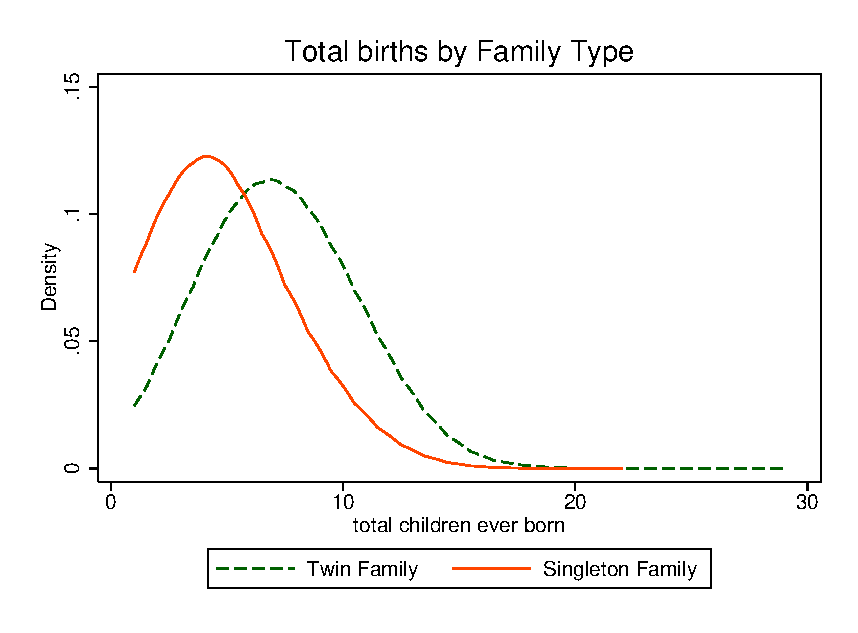
\includegraphics[scale=0.75]{./figures/famsize.eps}
\end{figure}
\hyperlink{Fstage}{\beamergotobutton{Regression}}
\end{frame}


%================================================================================
%==IV  Estimates- 2nd stage - DHS and NHIS
%================================================================================

\begin{frame}[label=IV]
\begin{landscape}\begin{table}[htpb!]\caption{Principal IV Results}
\label{TWINtab:IVAll}
\begin{center}\begin{tabular}{lcccp{2mm}cccp{2mm}ccc}
\toprule \toprule 
&\multicolumn{3}{c}{2+}&&\multicolumn{3}{c}{3+}&&\multicolumn{3}{c}{4+}\\ \cmidrule(r){2-4} \cmidrule(r){6-8} \cmidrule(r){10-12} 
\textsc{School Z-Score}&Base&+H&+S\&H&&Base&+H&+S\&H&&Base&+H&+S\&H\\ \midrule 
\begin{footnotesize}\end{footnotesize}& 
\begin{footnotesize}\end{footnotesize}& 
\begin{footnotesize}\end{footnotesize}& 
\begin{footnotesize}\end{footnotesize}& 
\begin{footnotesize}\end{footnotesize}& 
\begin{footnotesize}\end{footnotesize}& 
\begin{footnotesize}\end{footnotesize}& 
\begin{footnotesize}\end{footnotesize}& 
\begin{footnotesize}\end{footnotesize}& 
\begin{footnotesize}\end{footnotesize}& 
\begin{footnotesize}\end{footnotesize}& 
\begin{footnotesize}\end{footnotesize}\\ 
\multicolumn{12}{l}{\textbf{All}}\\ 
Fertility&0.006&-0.026&-0.026&&-0.004&-0.036&-0.038*&&-0.017&-0.036&-0.035*\\
&(0.029)&(0.027)&(0.026)&&(0.024)&(0.022)&(0.021)&&(0.025)&(0.023)&(0.021)\\
\begin{footnotesize}\end{footnotesize}&\begin{footnotesize}\end{footnotesize}&\begin{footnotesize}\end{footnotesize}&\begin{footnotesize}\end{footnotesize}&\begin{footnotesize}\end{footnotesize}&\begin{footnotesize}\end{footnotesize}&\begin{footnotesize}\end{footnotesize}&\begin{footnotesize}\end{footnotesize}&\begin{footnotesize}\end{footnotesize}&\begin{footnotesize}\end{footnotesize}&\begin{footnotesize}\end{footnotesize}&\begin{footnotesize}\end{footnotesize}\\Observations&249536&249536&249536&&375987&375987&375987&&385389&385389&385389\\
\multicolumn{12}{l}{\textbf{Low-Income}}\\ 
Fertility&0.035&0.008&0.012&&0.016&-0.016&-0.027&&-0.011&-0.031&-0.024\\
&(0.034)&(0.032)&(0.031)&&(0.030)&(0.028)&(0.026)&&(0.029)&(0.027)&(0.025)\\
\begin{footnotesize}\end{footnotesize}&\begin{footnotesize}\end{footnotesize}&\begin{footnotesize}\end{footnotesize}&\begin{footnotesize}\end{footnotesize}&\begin{footnotesize}\end{footnotesize}&\begin{footnotesize}\end{footnotesize}&\begin{footnotesize}\end{footnotesize}&\begin{footnotesize}\end{footnotesize}&\begin{footnotesize}\end{footnotesize}&\begin{footnotesize}\end{footnotesize}\\Observations&149602&149602&149602&&232371&232371&232371&&246622&246622&246622\\
\multicolumn{12}{l}{\textbf{Middle-Income}}\\ 
Fertility&-0.065&-0.087*&-0.093**&&-0.046&-0.079**&-0.067*&&-0.027&-0.048&-0.054\\
&(0.053)&(0.049)&(0.047)&&(0.040)&(0.036)&(0.035)&&(0.043)&(0.040)&(0.037)\\
\begin{footnotesize}\end{footnotesize}&\begin{footnotesize}\end{footnotesize}&\begin{footnotesize}\end{footnotesize}&\begin{footnotesize}\end{footnotesize}&\begin{footnotesize}\end{footnotesize}&\begin{footnotesize}\end{footnotesize}&\begin{footnotesize}\end{footnotesize}&\begin{footnotesize}\end{footnotesize}&\begin{footnotesize}\end{footnotesize}&\begin{footnotesize}\end{footnotesize}\\Observations&99934&99934&99934&&143616&143616&143616&&138767&138767&138767\\
\multicolumn{12}{l}{\textbf{Adjusted Fertility}}\\ 
Fertility&0.017&-0.052&-0.055&&-0.013&-0.073*&-0.077*&&-0.033&-0.068&-0.066*\\
&(0.065)&(0.056)&(0.054)&&(0.047)&(0.043)&(0.040)&&(0.045)&(0.042)&(0.039)\\
\begin{footnotesize}\end{footnotesize}&\begin{footnotesize}\end{footnotesize}&\begin{footnotesize}\end{footnotesize}&\begin{footnotesize}\end{footnotesize}&\begin{footnotesize}\end{footnotesize}&\begin{footnotesize}\end{footnotesize}&\begin{footnotesize}\end{footnotesize}&\begin{footnotesize}\end{footnotesize}&\begin{footnotesize}\end{footnotesize}&\begin{footnotesize}\end{footnotesize}\\Observations&249505&249505&249505&&375957&375957&375957&&385363&385363&385363\\
\multicolumn{12}{l}{\textbf{Twins and Pre-Twins}}\\ 
Fertility&-0.021&-0.073***&-0.078***&&-0.019&-0.062***&-0.067***&&-0.018&-0.039**&-0.046**\\
&(0.024)&(0.021)&(0.020)&&(0.020)&(0.018)&(0.018)&&(0.021)&(0.019)&(0.018)\\
\begin{footnotesize}\end{footnotesize}&\begin{footnotesize}\end{footnotesize}&\begin{footnotesize}\end{footnotesize}&\begin{footnotesize}\end{footnotesize}&\begin{footnotesize}\end{footnotesize}&\begin{footnotesize}\end{footnotesize}&\begin{footnotesize}\end{footnotesize}&\begin{footnotesize}\end{footnotesize}&\begin{footnotesize}\end{footnotesize}&\begin{footnotesize}\end{footnotesize}\\Observations&488815&488815&488815&&563177&563177&563177&&523197&523197&523197\\

\midrule\multicolumn{12}{p{19.2cm}}{\begin{footnotesize}\textsc{Notes:} The two plus subsample refers to all first born children in families with at least two births.  Three plus refers to first- and second-borns in families with at least three births, and four plus refers to first- to third-borns in families with at least four births.  Each cell presents the coefficient of a 2SLS regression where fertility is instrumented by twinning at birth order two, three or four (for 2+, 3+ and 4+ respectively).  Different rows of the table correspond to different sub-groups or specifications. In order these correspond to: all children, grouped by country income status, adjusting fertility to correct exclude children who did not survive to one year, and including both pre-twins \emph{and} twins in the regression. Base controls include child age, mother's age, and mother's age at birth fixed effects plus country and year-of-birth FEs.  In each case the sample is made up of all children aged between 6-18 years from families in the DHS who fulfill 2+ to 4+ requirements. First-stage results in the final panel correspond to the second stage in row 1. Full first stage results for each row are available in table \ref{TWINtab:FS}. Standard errors are clustered by mother.$^{*}$p$<$0.1; $^{**}$p$<$0.05; $^{***}$p$<$0.01 
\end{footnotesize}} \\ \bottomrule 
\end{tabular}\end{center}\end{table}\end{landscape}
\hyperlink{Fstage2}{\beamergotobutton{First stage}}
\end{frame}


\frame{\frametitle{IV Results by Gender}
\begin{table}[htpb!]\caption{Q-Q IV Estimates by Gender} 
\label{TWINtab:gend}\vspace{-5mm}\begin{center}\begin{tabular}{lcccccc}
\toprule \toprule 
&\multicolumn{3}{c}{Females}&\multicolumn{3}{c}{Males}\\ 
\cmidrule(r){2-4} \cmidrule(r){5-7} 
&Base&Socioec&Health&Base&Socioec&Health \\ \midrule 
\begin{footnotesize}\end{footnotesize}&\begin{footnotesize}\end{footnotesize}&\begin{footnotesize}\end{footnotesize}&\begin{footnotesize}\end{footnotesize}&\begin{footnotesize}\end{footnotesize}&\begin{footnotesize}\end{footnotesize}&\\Two Plus &0.014&-0.018&-0.023&-0.008&-0.027&-0.027\\
&(0.040)&(0.036)&(0.035)&(0.038)&(0.034)&(0.034)\\
\begin{footnotesize}\end{footnotesize}&\begin{footnotesize}\end{footnotesize}&\begin{footnotesize}\end{footnotesize}&\begin{footnotesize}\end{footnotesize}&\begin{footnotesize}\end{footnotesize}&\begin{footnotesize}\end{footnotesize}&\\Three Plus &-0.020&-0.047*&-0.050*&0.001&-0.028&-0.033\\
&(0.032)&(0.028)&(0.028)&(0.029)&(0.027)&(0.027)\\
\begin{footnotesize}\end{footnotesize}&\begin{footnotesize}\end{footnotesize}&\begin{footnotesize}\end{footnotesize}&\begin{footnotesize}\end{footnotesize}&\begin{footnotesize}\end{footnotesize}&\begin{footnotesize}\end{footnotesize}&\\Four Plus &-0.036&-0.051**&-0.056**&0.003&-0.007&-0.010\\
&(0.030)&(0.026)&(0.026)&(0.030)&(0.027)&(0.027)\\
\midrule\multicolumn{7}{p{11.5cm}}{\begin{footnotesize}\textsc{Notes:} Female or male refers to the gender of the index child of the regression. 
Sample sizes are, respectively 126,527, 131,716, 194,176, 196,809, 201,174, 201,950 for female and male two plus, F and M 
three plus and F and M four plus groups.  Additional controls are listed in 
the notes to table \ref{TWINtab:IVTwoplus}.  Standard errors are clustered 
by mother.$^{*}$p$<$0.1; $^{**}$p$<$0.05; $^{***}$p$<$0.01
\end{footnotesize}} \\ \bottomrule 
\end{tabular}\end{center}\end{table}
}


%%Damian can you bring NHIS IV results here for 2nd stage (with the 1st stage and OLS removed into separate tables please?)
\begin{frame}[label=USAIV]
\begin{table}[htpb!]\caption{NHIS Estimates (USA): Education and Health}
\label{TWINtab:NHISAll}
\begin{center}
\scalebox{0.52}{
\begin{tabular}{lcccp{2mm}cccp{2mm}ccc}
\toprule \toprule 
&\multicolumn{3}{c}{2+}&&\multicolumn{3}{c}{3+}&&\multicolumn{3}{c}{4+}\\ \cmidrule(r){2-4} \cmidrule(r){6-8} \cmidrule(r){10-12} 
&Base&+H&+S\&H&&Base&+H&+S\&H&&Base&+H&+S\&H\\ \midrule 
\begin{footnotesize}\end{footnotesize}& 
\begin{footnotesize}\end{footnotesize}& 
\begin{footnotesize}\end{footnotesize}& 
\begin{footnotesize}\end{footnotesize}& 
\begin{footnotesize}\end{footnotesize}& 
\begin{footnotesize}\end{footnotesize}& 
\begin{footnotesize}\end{footnotesize}& 
\begin{footnotesize}\end{footnotesize}& 
\begin{footnotesize}\end{footnotesize}& 
\begin{footnotesize}\end{footnotesize}& 
\begin{footnotesize}\end{footnotesize}& 
\begin{footnotesize}\end{footnotesize}\\ 
\multicolumn{12}{l}{\textbf{OLS}}\\ 
School Z-Score&-0.043***&-0.033***&-0.027***&&-0.036***&-0.028***&-0.020**&&-0.010&-0.004&0.002\\
&(0.005)&(0.006)&(0.006)&&(0.008)&(0.009)&(0.009)&&(0.018)&(0.018)&(0.018)-\\
Excellent Health&-0.012***&-0.005***&-0.004*&&-0.018***&-0.010***&-0.008***&&-0.028***&-0.019***&-0.017***\\
&(0.002)&(0.002)&(0.002)&&(0.004)&(0.003)&(0.003)&&(0.006)&(0.005)&(0.005)\\

\begin{footnotesize}\end{footnotesize}&\begin{footnotesize}\end{footnotesize}&\begin{footnotesize}\end{footnotesize}&\begin{footnotesize}\end{footnotesize}&\begin{footnotesize}\end{footnotesize}&\begin{footnotesize}\end{footnotesize}&\begin{footnotesize}\end{footnotesize}&\begin{footnotesize}\end{footnotesize}&\begin{footnotesize}\end{footnotesize}&\begin{footnotesize}\end{footnotesize}&\begin{footnotesize}\end{footnotesize}&\begin{footnotesize}\end{footnotesize}\\
\multicolumn{12}{l}{\textbf{IV}}\\ 
School Z-Score&-0.064&-0.074&-0.077&&-0.027&-0.037&-0.036&&-0.094&-0.099&-0.113\\
&(0.063)&(0.059)&(0.058)&&(0.065)&(0.064)&(0.065)&&(0.152)&(0.155)&(0.150)\\

Excellent Health&0.013&0.022&0.019&&-0.016&-0.054*&-0.055*&&0.057&0.017&0.006\\
&(0.025)&(0.020)&(0.020)&&(0.038)&(0.031)&(0.031)&&(0.058)&(0.054)&(0.052)\\
\begin{footnotesize}\end{footnotesize}&\begin{footnotesize}\end{footnotesize}&\begin{footnotesize}\end{footnotesize}&\begin{footnotesize}\end{footnotesize}&\begin{footnotesize}\end{footnotesize}&\begin{footnotesize}\end{footnotesize}&\begin{footnotesize}\end{footnotesize}&\begin{footnotesize}\end{footnotesize}&\begin{footnotesize}\end{footnotesize}&\begin{footnotesize}\end{footnotesize}&\begin{footnotesize}\end{footnotesize}&\begin{footnotesize}\end{footnotesize}\\
\multicolumn{12}{l}{\textbf{Descriptives}}\\ 
School Z-Score&-0.0233&&&&-0.0363&&&&-0.0628&&\\
&(0.993)&&&&(1.041)&&&&(1.086)&&\\
Excellent Health&0.533&&&&0.511&&&&0.490&&\\
&(0.499)&&&&(0.500)&&&&(0.500)&&\\
\begin{footnotesize}\end{footnotesize}&\begin{footnotesize}\end{footnotesize}&\begin{footnotesize}\end{footnotesize}&\begin{footnotesize}\end{footnotesize}&\begin{footnotesize}\end{footnotesize}&\begin{footnotesize}\end{footnotesize}&\begin{footnotesize}\end{footnotesize}&\begin{footnotesize}\end{footnotesize}&\begin{footnotesize}\end{footnotesize}&\begin{footnotesize}\end{footnotesize}&\begin{footnotesize}\end{footnotesize}&\begin{footnotesize}\end{footnotesize}\\ 
Observations & 75,902 &	75,902 &	75,902 &&	57,413 &	57,413 &	57,413 &&	26,128 &	26,128 &	26,128 \\
Joint F-test Educ &&164.5&64.7&&&101.3&39.6&&&38.0&7.7\\
Joint F-test Health &&34469.6&163.9&&&15335.6&28.4&&&5276.4&17.1\\
\midrule\multicolumn{12}{p{20.6cm}}{\begin{footnotesize}\textsc{Notes:}  
Each cell presents the coefficient of interest from a regression using NHIS survey data (2002-2014). Base controls include child age FE (in months), mother's age, and mother's age at first birth 
plus race dummies for child and mother.  First stage omitted for clarity (generally all around 0.7).  Standard errors are clustered by mother.$^{*}$p$<$0.1; $^{**}$p$<$0.05; $^{***}$p$<$0.01. 
\end{footnotesize}} \\ \bottomrule 
\end{tabular}}\end{center}\end{table}

\end{frame}

%% Damian i have stopped editing at this point today and will continue tomorrow. You can see the drift of my restructuring.

%% Damian could you add a nicer, systematic discussion of Conley's method and our approach to estimation of gamma in USA and Nigeria somewhere here.
%%RESPONSE: I will aim to set out estimation pieces this weekend for both the paper and the slides.  I will follow your outline in the email with planned structure from 19 May 2016.

%================================================================================
%== Summary of OLS and IV estimates
%================================================================================

\frame{\frametitle{Summary: OLS and\ IV}
\begin{itemize}
\item Education, developing countries: OLS $-0.08^{*}$ (parity pooled), smaller conditional on mother characteristics. 
\item IV $-0.04^{*}$ (3+, all) to $-0.06^{*}$ (3+, middle income), larger conditional on mother characteristics. 
\end{itemize}       \\ \vspace{5mm}

%%Damian we need to add the effect sizes here, if in paper i will add in next round. Need to be sure i know the units/ if standardized
\begin{itemize}
\item Education, USA: OLS xxxx estimates with/without conditioning 
\item IV xxxx estimates with/without conditioning
\item Health, USA OLS xxxx estimates with/without conditioning
\item IV xxxx estimates with/without conditioning
\end{itemize}
\item First stage indicates twin birth is a powerful instrument, coefficient 0.8 in developing countries, 0.xx in USA. 
\end{itemize}
}



%================================================================================
%== Bounds - idea
%================================================================================

\frame{
\begin{center}
\Large Estimating Bounds on the IV Estimates
\end{center}
}

\frame{\frametitle{Plausible exogeneity}
An approach to inference for IV models with instruments whose validity is debatable.
\[
schooling = \beta fertility + \textcolor{red}{\gamma twins} + X\delta+ e
\]
\begin{itemize}
\item Relax the exclusion restriction that $\gamma=0$.
\item Plausible exogeneity corresponds to having prior information that $\gamma$ is near 0 but not exactly 0 (Conley et al.\ 2012)
\item The 2SLS estimator is less sensitive to violations of the exclusion restriction when the instrument is strong (related, Bound, Jaeger, Baker 1995). \ Ours is such a case.
\item Similar strategy in Nevo and Rosen (2012).
\end{itemize}
}

%================================================================================
%== Bounds - Conley procedures
%================================================================================

%%Damian is going to rewrite the next few slides and add one each on the procedures for estimating gamma from nigeria and usasulfa data.

\frame{\frametitle{Procedures}
Conley et al. 2012 present four complementary inference strategies that use prior information about $\gamma$ to different extents. We implement two of these: union of confidence interval (UCI) and the local to zero approach (LTZ)
\vspace{4mm}
\begin{itemize}
\item We specify a set of plausible values for $\gamma$ and obtain interval estimates for $\beta$ conditional upon each.  Grid over 0 to 2$\hat\gamma$.
\item Taking the union of these interval estimates across values of $\gamma$ provides a conservative interval estimate for $\beta$.
\begin{itemize}
\item The plus is that we don’t need to specify a prior distribution for $\gamma$, just a range of plausible values.
\item The minus is that the estimated interval around $\beta$ may be wide
\end{itemize}
\item The LTZ approach views prior probabilities for $\gamma$ as analogous to objective probabilities in a 2-step DGP.  Here we must specificy a prior distribution.
\end{itemize}
}

================================================================================
%== Bounds - Conley Results
%================================================================================

%%Damian to add results not only on bounds as below but also on the 2 components of gamma, the plot of the distribution.. maybe with hyperlinks going fwd and back.

\frame{\frametitle{Estimates of bounds: UCI and LTZ Approaches}
\begin{table}[htpb!]\caption{`Plausibly Exogenous' Bounds} 
\label{TWINtab:Conley}\vspace{-5mm}\begin{center}\begin{tabular}{lcccc}
\toprule \toprule 
&\multicolumn{2}{c}{UCI: $\gamma\in [0,\delta]$}&\multicolumn{2}{c}{LTZ: $\gamma \sim U(0,\delta)$}\\ 
\cmidrule(r){2-3} \cmidrule(r){4-5}
&Lower Bound&Upper Bound&Lower Bound&Upper Bound\\
Two Plus&-0.1827&0.0173&-0.1584&-0.0008\\
Three Plus&-0.1659&-0.0019&-0.1485&-0.0155\\
Four Plus&-0.1486&-0.0062&-0.1332&-0.0186\\
Five Plus&-0.1329&0.0203&-0.1182&0.0076\\
\midrule\multicolumn{5}{p{11.6cm}}{\begin{footnotesize}\textsc{Notes:} This table presents upper and lower bounds of a 95\% confidence interval for the effects of family size on (standardised) children's education attainment. These are estimated by the methodology of \citet{Conleyetal2012}  under various priors about the direct effect that being from a twin family has on educational outcomes ($\gamma$). In the UCI (union of confidence interval) approach, it is assumed the true $\gamma\in[0,\delta]$, while in the LTZ (local to zero) approach it is assumed that $\gamma\sim U(0,\delta)$.  In each case $\delta$ is estimated by including twinning in the first stage  equation and observing the effect size $\hat\gamma$.  Estimated $\hat\gamma$'s are (respectively for two plus to five plus):   0.1077, 0.0931, 0.0810, 0.0870.\end{footnotesize}}  
\\ \bottomrule \end{tabular}\end{center}\end{table} 

}

\frame{\frametitle{Estimates (3+) Assuming that $\gamma \sim U(0,\delta)$}
\begin{figure}[htpb!]
\centering
  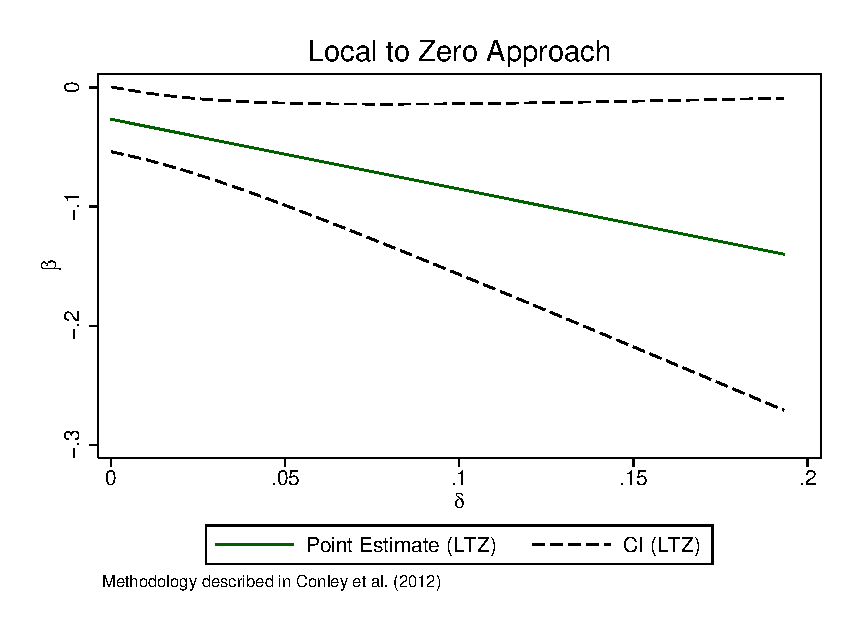
\includegraphics[scale=0.75]{./figures/LTZ_three.eps}
\end{figure}
\hyperlink{2+}{\beamergotobutton{two}}\ \hyperlink{4+}{\beamergotobutton{four}}
}


%================================================================================
%== Slide 32: Conclusions
%================================================================================
\section{Conclusions}
\frame{\frametitle{Conclusions}
\begin{itemize}
\item Indicators of mother's health and pregnancy behaviours are significant predictors of twin birth.\\ \vspace{5mm}
\item Conditioning upon available twin predictors produces evidence of a trade-off in IV ($\sim -0.04$ s.d.) and RF estimates.\\ \vspace{5mm}
\item Recognizing that twins are at best plausibly exogenous results in a QQ parameter interval with an upper bound of $\sim -0.15$ s.d. \\ \vspace{5mm}
\item Significantly larger trade-off for middle income countries and for female children\\ \vspace{5mm}
\item Ignoring the twin bias will similarly tend to lead to under-estimation of the trade-off between fertility and women's labour force participation.
\end{itemize}
}


% Summary stats for DHS
% Damian can you add under this the summ stats table for NHIS we have in the paper
%%RESPONSE: Yes, I will bring in the NHIS results.
\frame{
\begin{table}[htpb!]\caption{Summary Statistics} 
\label{TWINtab:sumstats}\begin{center}\scalebox{0.6}{\begin{tabular}{lccccc}
\toprule \toprule 
&\multicolumn{2}{c}{Low Income}&\multicolumn{2}{c}{Middle Income}\\ 
\cmidrule(r){2-3} \cmidrule(r){4-5}
& Single & Twins & Single & Twins & All \\ \midrule 
\textsc{Fertility} & & & & & \\ 
Fertility&3.670&6.093&3.348&5.425&3.609\\
&(2.365)&(2.582)&(2.272)&(2.609)&(2.372)\\
Desired Family Size&4.182&5.296&3.340&4.128&3.892\\
&(2.500)&(2.832)&(2.083)&(2.498)&(2.403)\\
Fraction Twin & \multicolumn{2}{c}{  0.0194}& \multicolumn{2}{c}{  0.0173 } &  0.0185\\
& \multicolumn{2}{c}{(0.1379)}& \multicolumn{2}{c}{(0.1306)} & (0.1348)\\
\textsc{Health of Mother}&&&&&\\ 
Height&155.6&157.7&155.6&157.2&155.7\\
&(7.084)&(6.987)&(6.956)&(6.957)&(7.042)\\
BMI&21.89&22.47&25.83&26.50&23.38\\
&(3.983)&(4.098)&(5.066)&(5.437)&(4.822)\\
Pr(BMI)$<$18.5&0.172&0.123&0.0344&0.0276&0.119\\
&(0.377)&(0.328)&(0.182)&(0.164)&(0.324)\\
\textsc{Children's Outcomes}&&&&&\\ Education (Years)
&3.695&3.212&5.438&4.999&4.465\\
&(3.581)&(3.270)&(3.859)&(3.734)&(3.805)\\
Education (Z-Score)&-0.00869&-0.0130&0.0121&-0.0366&0.000177\\
&(1.001)&(0.961)&(0.998)&(0.987)&(1.000)\\
\midrule
Number of Countries &42&42&34&34&68 \\
Number of Mothers &491,905 &7,457 &297,413 &4,317 & 850,032 \\
Number of Children (Education) &1,176,513 &25,003 &714,751 &14,333 & 1,930,600 \\
Number of Children (Ever Born) &1,716,247 &43,866 &940,204 &21,302 & 2,721,619 \\
\midrule
\multicolumn{6}{p{13.8cm}}{\begin{footnotesize}\textsc{Notes:} Group means (sd).\end{footnotesize}} \\ \bottomrule \end{tabular}}\end{center}\end{table}

}



\section{Appendices}
\frame{
\begin{center}
\Large \textcolor{blue}{Appendices}
\end{center}
}

\frame{
\begin{center}
\Large \textcolor{blue}{Appendix Tables}
\end{center}
}

\begin{frame}[label=Fstage]
\frametitle{First Stage: Twins Increase Family Size by $\sim$0.8}
\begin{landscape}\begin{table}[htpb!]\caption{First Stage Results} 
\label{TWINtab:FS}\begin{center}\begin{tabular}{lccccccccc}
\toprule \toprule 
&\multicolumn{3}{c}{2+}&\multicolumn{3}{c}{3+}&\multicolumn{3}{c}{4+}\\ \cmidrule(r){2-4} \cmidrule(r){5-7} \cmidrule(r){8-10} 
\textsc{Fertility}&Base&+S&+S\&H&Base&+S&+S\&H&Base&+S&+S\&H\\ \midrule 
\begin{footnotesize}\end{footnotesize}& 
\begin{footnotesize}\end{footnotesize}& 
\begin{footnotesize}\end{footnotesize}& 
\begin{footnotesize}\end{footnotesize}& 
\begin{footnotesize}\end{footnotesize}& 
\begin{footnotesize}\end{footnotesize}& 
\begin{footnotesize}\end{footnotesize}& 
\begin{footnotesize}\end{footnotesize}& 
\begin{footnotesize}\end{footnotesize}& 
\begin{footnotesize}\end{footnotesize}\\ 
\multicolumn{10}{l}{\textbf{Pre-Twins}}\\ 
Twin&0.798***&0.839***&0.841***&0.796***&0.821***&0.824***&0.841***&0.860***&0.863***\\
&(0.030)&(0.028)&(0.028)&(0.027)&(0.026)&(0.026)&(0.027)&(0.026)&(0.026)\\
\begin{footnotesize}\end{footnotesize}&\begin{footnotesize}\end{footnotesize}&\begin{footnotesize}\end{footnotesize}&\begin{footnotesize}\end{footnotesize}&\begin{footnotesize}\end{footnotesize}&\begin{footnotesize}\end{footnotesize}&\begin{footnotesize}\end{footnotesize}&\begin{footnotesize}\end{footnotesize}&\begin{footnotesize}\end{footnotesize}&\begin{footnotesize}\end{footnotesize}\\\multicolumn{10}{l}{\textbf{Pre-Twins (+bord)}}\\ 
Twin&0.796***&0.838***&0.839***&0.793***&0.825***&0.828***&0.842***&0.863***&0.865***\\
&(0.030)&(0.028)&(0.028)&(0.027)&(0.026)&(0.026)&(0.026)&(0.026)&(0.026)\\
\begin{footnotesize}\end{footnotesize}&\begin{footnotesize}\end{footnotesize}&\begin{footnotesize}\end{footnotesize}&\begin{footnotesize}\end{footnotesize}&\begin{footnotesize}\end{footnotesize}&\begin{footnotesize}\end{footnotesize}&\begin{footnotesize}\end{footnotesize}&\begin{footnotesize}\end{footnotesize}&\begin{footnotesize}\end{footnotesize}&\begin{footnotesize}\end{footnotesize}\\\multicolumn{10}{l}{\textbf{Low-Income}}\\ 
Twin&0.844***&0.861***&0.861***&0.804***&0.822***&0.824***&0.863***&0.866***&0.868***\\
&(0.037)&(0.036)&(0.036)&(0.033)&(0.032)&(0.032)&(0.032)&(0.032)&(0.032)\\
\begin{footnotesize}\end{footnotesize}&\begin{footnotesize}\end{footnotesize}&\begin{footnotesize}\end{footnotesize}&\begin{footnotesize}\end{footnotesize}&\begin{footnotesize}\end{footnotesize}&\begin{footnotesize}\end{footnotesize}&\begin{footnotesize}\end{footnotesize}&\begin{footnotesize}\end{footnotesize}&\begin{footnotesize}\end{footnotesize}&\begin{footnotesize}\end{footnotesize}\\\multicolumn{10}{l}{\textbf{Middle-Income}}\\ 
Twin&0.741***&0.803***&0.806***&0.774***&0.810***&0.815***&0.790***&0.844***&0.846***\\
&(0.051)&(0.045)&(0.045)&(0.047)&(0.044)&(0.044)&(0.047)&(0.043)&(0.043)\\
\begin{footnotesize}\end{footnotesize}&\begin{footnotesize}\end{footnotesize}&\begin{footnotesize}\end{footnotesize}&\begin{footnotesize}\end{footnotesize}&\begin{footnotesize}\end{footnotesize}&\begin{footnotesize}\end{footnotesize}&\begin{footnotesize}\end{footnotesize}&\begin{footnotesize}\end{footnotesize}&\begin{footnotesize}\end{footnotesize}&\begin{footnotesize}\end{footnotesize}\\\multicolumn{10}{l}{\textbf{Desired-Threshold}}\\ 
Twin&0.775***&0.821***&0.822***&0.749***&0.786***&0.788***&0.846***&0.863***&0.865***\\
&(0.036)&(0.033)&(0.033)&(0.030)&(0.029)&(0.029)&(0.028)&(0.028)&(0.028)\\
Twin$\times$desire&0.085&0.064&0.066&0.220***&0.161**&0.165**&-0.031&-0.016&-0.011\\
&(0.067)&(0.062)&(0.062)&(0.070)&(0.066)&(0.066)&(0.085)&(0.079)&(0.080)\\
\begin{footnotesize}\end{footnotesize}&\begin{footnotesize}\end{footnotesize}&\begin{footnotesize}\end{footnotesize}&\begin{footnotesize}\end{footnotesize}&\begin{footnotesize}\end{footnotesize}&\begin{footnotesize}\end{footnotesize}&\begin{footnotesize}\end{footnotesize}&\begin{footnotesize}\end{footnotesize}&\begin{footnotesize}\end{footnotesize}&\begin{footnotesize}\end{footnotesize}\\\multicolumn{10}{l}{\textbf{Twins and Pre-twins}}\\ 
Twin&0.747***&0.801***&0.806***&0.815***&0.831***&0.835***&0.861***&0.863***&0.868***\\
&(0.028)&(0.026)&(0.026)&(0.028)&(0.027)&(0.027)&(0.027)&(0.026)&(0.026)\\
\begin{footnotesize}\end{footnotesize}&\begin{footnotesize}\end{footnotesize}&\begin{footnotesize}\end{footnotesize}&\begin{footnotesize}\end{footnotesize}&\begin{footnotesize}\end{footnotesize}&\begin{footnotesize}\end{footnotesize}&\begin{footnotesize}\end{footnotesize}&\begin{footnotesize}\end{footnotesize}&\begin{footnotesize}\end{footnotesize}&\begin{footnotesize}\end{footnotesize}\\
\midrule\multicolumn{10}{p{18.0cm}}{\begin{footnotesize}\textsc{Notes:} Each cell represents the coefficient from the first-stage of a two-stage regression.  The first-stage represents the effect of twinning at parity $N$ on total fertility where $N$ is 2, 3 or 4 for 2+, 3+ and 4+ groups respectively.  The 2+ group includes all first borns in families with at least 2 births, the 3+ group includes first and second borns in families with at least 3 births, and the 4+ group includes all first to third borns in families with at least four births.  In each regressions the sample is made up of all children aged between 6-18 years from families in the DHS who fulfill these birth order conditions.  Controls in each case are identical to those described in table \ref{TWINtab:IVTwoplus}.  Standard errors are clustered at the level of the mother.$^{*}$p$<$0.1; $^{**}$p$<$0.05; $^{***}$p$<$0.01 
\end{footnotesize}} \\ \bottomrule 
\end{tabular}\end{center}\end{table}\end{landscape}
\hyperlink{FS1}{\beamergotobutton{Back}}
\end{frame}

\begin{frame}[label=Fstage2]
\frametitle{First Stage: Twins Increase Family Size by $\sim$0.8}
\begin{landscape}\begin{table}[htpb!]\caption{First Stage Results} 
\label{TWINtab:FS}\begin{center}\begin{tabular}{lccccccccc}
\toprule \toprule 
&\multicolumn{3}{c}{2+}&\multicolumn{3}{c}{3+}&\multicolumn{3}{c}{4+}\\ \cmidrule(r){2-4} \cmidrule(r){5-7} \cmidrule(r){8-10} 
\textsc{Fertility}&Base&+S&+S\&H&Base&+S&+S\&H&Base&+S&+S\&H\\ \midrule 
\begin{footnotesize}\end{footnotesize}& 
\begin{footnotesize}\end{footnotesize}& 
\begin{footnotesize}\end{footnotesize}& 
\begin{footnotesize}\end{footnotesize}& 
\begin{footnotesize}\end{footnotesize}& 
\begin{footnotesize}\end{footnotesize}& 
\begin{footnotesize}\end{footnotesize}& 
\begin{footnotesize}\end{footnotesize}& 
\begin{footnotesize}\end{footnotesize}& 
\begin{footnotesize}\end{footnotesize}\\ 
\multicolumn{10}{l}{\textbf{Pre-Twins}}\\ 
Twin&0.798***&0.839***&0.841***&0.796***&0.821***&0.824***&0.841***&0.860***&0.863***\\
&(0.030)&(0.028)&(0.028)&(0.027)&(0.026)&(0.026)&(0.027)&(0.026)&(0.026)\\
\begin{footnotesize}\end{footnotesize}&\begin{footnotesize}\end{footnotesize}&\begin{footnotesize}\end{footnotesize}&\begin{footnotesize}\end{footnotesize}&\begin{footnotesize}\end{footnotesize}&\begin{footnotesize}\end{footnotesize}&\begin{footnotesize}\end{footnotesize}&\begin{footnotesize}\end{footnotesize}&\begin{footnotesize}\end{footnotesize}&\begin{footnotesize}\end{footnotesize}\\\multicolumn{10}{l}{\textbf{Pre-Twins (+bord)}}\\ 
Twin&0.796***&0.838***&0.839***&0.793***&0.825***&0.828***&0.842***&0.863***&0.865***\\
&(0.030)&(0.028)&(0.028)&(0.027)&(0.026)&(0.026)&(0.026)&(0.026)&(0.026)\\
\begin{footnotesize}\end{footnotesize}&\begin{footnotesize}\end{footnotesize}&\begin{footnotesize}\end{footnotesize}&\begin{footnotesize}\end{footnotesize}&\begin{footnotesize}\end{footnotesize}&\begin{footnotesize}\end{footnotesize}&\begin{footnotesize}\end{footnotesize}&\begin{footnotesize}\end{footnotesize}&\begin{footnotesize}\end{footnotesize}&\begin{footnotesize}\end{footnotesize}\\\multicolumn{10}{l}{\textbf{Low-Income}}\\ 
Twin&0.844***&0.861***&0.861***&0.804***&0.822***&0.824***&0.863***&0.866***&0.868***\\
&(0.037)&(0.036)&(0.036)&(0.033)&(0.032)&(0.032)&(0.032)&(0.032)&(0.032)\\
\begin{footnotesize}\end{footnotesize}&\begin{footnotesize}\end{footnotesize}&\begin{footnotesize}\end{footnotesize}&\begin{footnotesize}\end{footnotesize}&\begin{footnotesize}\end{footnotesize}&\begin{footnotesize}\end{footnotesize}&\begin{footnotesize}\end{footnotesize}&\begin{footnotesize}\end{footnotesize}&\begin{footnotesize}\end{footnotesize}&\begin{footnotesize}\end{footnotesize}\\\multicolumn{10}{l}{\textbf{Middle-Income}}\\ 
Twin&0.741***&0.803***&0.806***&0.774***&0.810***&0.815***&0.790***&0.844***&0.846***\\
&(0.051)&(0.045)&(0.045)&(0.047)&(0.044)&(0.044)&(0.047)&(0.043)&(0.043)\\
\begin{footnotesize}\end{footnotesize}&\begin{footnotesize}\end{footnotesize}&\begin{footnotesize}\end{footnotesize}&\begin{footnotesize}\end{footnotesize}&\begin{footnotesize}\end{footnotesize}&\begin{footnotesize}\end{footnotesize}&\begin{footnotesize}\end{footnotesize}&\begin{footnotesize}\end{footnotesize}&\begin{footnotesize}\end{footnotesize}&\begin{footnotesize}\end{footnotesize}\\\multicolumn{10}{l}{\textbf{Desired-Threshold}}\\ 
Twin&0.775***&0.821***&0.822***&0.749***&0.786***&0.788***&0.846***&0.863***&0.865***\\
&(0.036)&(0.033)&(0.033)&(0.030)&(0.029)&(0.029)&(0.028)&(0.028)&(0.028)\\
Twin$\times$desire&0.085&0.064&0.066&0.220***&0.161**&0.165**&-0.031&-0.016&-0.011\\
&(0.067)&(0.062)&(0.062)&(0.070)&(0.066)&(0.066)&(0.085)&(0.079)&(0.080)\\
\begin{footnotesize}\end{footnotesize}&\begin{footnotesize}\end{footnotesize}&\begin{footnotesize}\end{footnotesize}&\begin{footnotesize}\end{footnotesize}&\begin{footnotesize}\end{footnotesize}&\begin{footnotesize}\end{footnotesize}&\begin{footnotesize}\end{footnotesize}&\begin{footnotesize}\end{footnotesize}&\begin{footnotesize}\end{footnotesize}&\begin{footnotesize}\end{footnotesize}\\\multicolumn{10}{l}{\textbf{Twins and Pre-twins}}\\ 
Twin&0.747***&0.801***&0.806***&0.815***&0.831***&0.835***&0.861***&0.863***&0.868***\\
&(0.028)&(0.026)&(0.026)&(0.028)&(0.027)&(0.027)&(0.027)&(0.026)&(0.026)\\
\begin{footnotesize}\end{footnotesize}&\begin{footnotesize}\end{footnotesize}&\begin{footnotesize}\end{footnotesize}&\begin{footnotesize}\end{footnotesize}&\begin{footnotesize}\end{footnotesize}&\begin{footnotesize}\end{footnotesize}&\begin{footnotesize}\end{footnotesize}&\begin{footnotesize}\end{footnotesize}&\begin{footnotesize}\end{footnotesize}&\begin{footnotesize}\end{footnotesize}\\
\midrule\multicolumn{10}{p{18.0cm}}{\begin{footnotesize}\textsc{Notes:} Each cell represents the coefficient from the first-stage of a two-stage regression.  The first-stage represents the effect of twinning at parity $N$ on total fertility where $N$ is 2, 3 or 4 for 2+, 3+ and 4+ groups respectively.  The 2+ group includes all first borns in families with at least 2 births, the 3+ group includes first and second borns in families with at least 3 births, and the 4+ group includes all first to third borns in families with at least four births.  In each regressions the sample is made up of all children aged between 6-18 years from families in the DHS who fulfill these birth order conditions.  Controls in each case are identical to those described in table \ref{TWINtab:IVTwoplus}.  Standard errors are clustered at the level of the mother.$^{*}$p$<$0.1; $^{**}$p$<$0.05; $^{***}$p$<$0.01 
\end{footnotesize}} \\ \bottomrule 
\end{tabular}\end{center}\end{table}\end{landscape}
\hyperlink{IV}{\beamergotobutton{Back}}
\end{frame}

 \begin{frame}[label=Spain1]
\begin{table}
\caption{Probability of Twin Birth: Spain Administrative Data 2007--2012}
\begin{center}
\scalebox{0.6}{
\begin{tabular}{lc}
\hline
VARIABLES	&	Twin*100 \\	\hline
	&	(1)	\\
Primary Education (Mother)	&	  -.04713**	\\
	&	 (0.02404)	\\
      Secondary Education (Mother)	&	  -.11682***	\\
	&	(0.02528)	\\
   Tertiary Education (Mother)	&	  -.03166	\\
	&	(0.02766)	\\
  Parents are Immigrants	&	  -.17078***	\\
	&	(0.03354)	\\
        citm	&	   .38144***	\\
	&	(0.03247)	\\
 Married	&	   .63864***	\\
	&	(0.01844)	\\
    Mother's Age	&	   1.63192***	\\
	&	(0.09688)	\\
    Mother's Age$^2$	&	  -.05818***	\\
	&	(0.00342)	\\
   Father's Age	&	  -.17344***	\\
	&	(0.04788)	\\
   Father's Age$^2$	&	   .00621***	\\
	&	(0.00137)	\\
   No Father	&	  -.48331	\\
	&	(0.53907)	\\
    Constant	&	  -13.20683	\\
	&	(0.94074)	\\
	& \\
	Observations & 2,869,329 \\
	$R^2$ & 0.0068 \\ \hline
\end{tabular}}
\end{center}
\end{table}

\hyperlink{c}{\beamergotobutton{Back}}
\end{frame}

 \begin{frame}[label=Brazil]
\begin{table}[htpb!]
\caption{Probability of Twin Births: Brazil Administrative Data}
\begin{center}
\scalebox{0.56}{

\begin{tabular}{llcc}\hline

&&(1)&(2)\\ \cmidrule(r){3-4}
&&\multicolumn{2}{c}{Probability for twin}\\ \hline
&&&\\

Female	&		&	0.0012***	&	0.0012***	\\
	&		&	(0.0001)	&	(0.0001)	\\
Age	&		&	0.0008***	&	0.0009***	\\
	&		&	(0.0000)	&	(0.0000)	\\
Marital status	&	Married	&	0.0008***	&	0.0009***	\\
	&		&	(0.0001)	&	(0.0001)	\\
	&	Divorced	&	0.0002	&	0.0002	\\
	&		&	(0.0006)	&	(0.0006)	\\
Years of schooling	&		&	-0.0000**	&	-0.0000**	\\
	&		&	(0.0000)	&	(0.0000)	\\
Number of live births&	&		0.0006***	&	0.0005***	\\
	&		&	(0.0000)	&	(0.0000)	\\
Number of still births&		&	-0.0001**	&	-0.0002***	\\
	&		&	(0.0001)	&	(0.0001)	\\
Race	&	Black	&	-0.0011***	&	-0.0014***	\\
	&		&	(0.0002)	&	(0.0002)	\\
	&	Asian	&	-0.0014***	&	-0.0019***	\\
	&		&	(0.0005)	&	(0.0005)	\\
	&	Mixed	&	-0.0016***	&	-0.0019***	\\
	&		&	(0.0001)	&	(0.0001)	\\
	&	Indigenous	&	-0.0057***	&	-0.0065***	\\
	&		&	(0.0004)	&	(0.0004)	\\
Number of prenatal visits	&		&		&	-0.0005***	\\
	&		&		&	(0.0000)	\\
Constant	&		&	-0.0035***	&	-0.0009***	\\
	&		&	(0.0001)	&	(0.0002)	\\
R-squared	&		&	0.0020	&	0.0021	\\ \hline
\multicolumn{4}{p{12cm}}{\begin{footnotesize}Notes: Standard errors are clustered at the municipality level. Number of observations = 20,013,814. *** $p<0.01$, ** $p<0.05$, * $p<0.1$ \end{footnotesize}}\\




\end{tabular}}


\end{center}
\end{table}

\hyperlink{c}{\beamergotobutton{Back}}
\end{frame}

\begin{frame}[label=Sweden]
\begin{table}[htpb!] 
\caption{Probability of Giving Birth to Twins (Sweden Birth Registry)} \label{TWINtab:twinregS} 
\begin{center}
\scalebox{0.64}{
\begin{tabular}{lccc} \toprule \toprule 
&(1)&(2)&(3)\\
Twin*100&All&\multicolumn{2}{c}{Time}\\
 \cmidrule(r){3-4} 
&&1991-2010&1983-1990\\\midrule
\begin{footnotesize}\end{footnotesize}&\begin{footnotesize}\end{footnotesize}&\begin{footnotesize}\end{footnotesize}&\begin{footnotesize}\end{footnotesize}\\
Age&0.257***&0.483***&0.277***\\
&(0.031)&(0.047)&(0.040)\\
Age Squared&-0.002***&-0.005***&-0.003***\\
&(0.001)&(0.001)&(0.001)\\
Education (years)&0.014&0.011&-0.013\\
&(0.009)&(0.014)&(0.012)\\
Height&0.038***&0.047***&0.019***\\
&(0.003)&(0.003)&(0.004)\\
Smoked&0.252***&0.237***&0.208***\\
&(0.045)&(0.069)&(0.056)\\
Alcohol&0.160&-2.381***&0.137\\
&(1.176)&(0.414)&(1.192)\\
&&&\\R-squared&0.01&0.01&0.01\\
Observations &1,628,737&1,098,076&530,661\\
\hline\hline\multicolumn{4}{p{8.3cm}}{\begin{footnotesize}\textsc{Notes:} Conditional on birth cohorts and marriage status FEs.  Linear probability estimates.  Standard errors in parenthesis are clustered at the level of the mother.
$^{*}$p$<$0.1; $^{**}$p$<$0.05; $^{***}$p$<$0.01
 \end{footnotesize}}\\ \hline \normalsize \end{tabular}}\end{center}\end{table} 

\hyperlink{c}{\beamergotobutton{Back}}
\end{frame}

\begin{frame}
\begin{table}
\caption{Twins, Miscarriage and Maternal Health (Administrative Data from Spain)}
\begin{center}
\scalebox{0.76}{
\begin{tabular}{lclc}
\hline 
VARIABLES	&	Fetal Death$	\times$100 & & \\	\hline
	&	(1) & &	\\
Primary	&	  -0.60179*** &	Primary$	\times$Twin	&	   -0.6618***	\\
	&	 (0.01456)	& &	 (0.20926)	\\
Secondary	&	  -0.71998*	& Secondary$	\times$Twin	&	  -0.55901***	\\
	&	  (0.0151)	& 	&	 .0020978	\\
Tertiary	&	  -0.80019***	& Tertiary$	\times$Twin	&	  -0.65091***	\\
	&	(0.01582)	& 	&	(0.20866)	\\
Immigration	&	  -0.07223***	& Immigration$	\times$Twin	&	  0.22871	\\
	&	 (0.0171)	& 	&	(0.29614)	\\
City	&	  -0.00321	& City$	\times$Twin	&	  0.09566	\\
	&	(0.01584)	& 	&	 (0.26876)	\\
Married	&	  -0.07354***	&Married$	\times$Twin	&	  -0.08978	\\
	&	 (0.00759)	&	&	 (0.11893)	\\
No Father	&	0.68626***	&No Father$	\times$Twin	&	3.25232	\\
	&	 (0.23825)	&	&	(4.09309)	\\
Constant	&	-1.35966***	& & \\
	&	(0.33674)	& &  \\
	& \\
	Obs & 2,869,329 & & \\
	$R^2$ & 0.0044  & & \\ \midrule
	\multicolumn{4}{p{8cm}}{Note: Spanish administrative births: 2007-2012.}
\end{tabular}}
\end{center}
\end{table}

\hyperlink{c}{\beamergotobutton{Back}}
\end{frame}

\begin{frame}[label=MMRselec]
\frametitle{Height and Selective Maternal Survival (1)} 
\begin{itemize}
\item We use unique data on maternal mortality rates of sisters of female respondents in the DHS.
\item We count the number of `unhealthy' women whose sisters died ($N_u$) and the number of `healthy' women whose sisters died ($N_h$).
\item We assume $N_u > N_h$ given that our data show that maternal mortality (of sisters) depends upon height (assumes height correlated across sisters).
\item First, we expand our sample to include $N_u + N_h$ women, choosing them randomly from within our file, based upon their `health'.
\item We use different measures of `health' to check sensitivity of results to this. We use different thresholds and combine being short and being underweight.
\end{itemize}
\end{frame}

\begin{frame}
\frametitle{Height and Selective Maternal Survival (2)}
\begin{itemize}
\item Second, we assume that the unhealthy women who died in childbirth were all carrying twins and that the healthy women who died in childbirth were all carrying singletons. 
\item This is an extreme assumption intended to produce a severe test of selection.
\item We then re-estimate the regression of prob(twin) on indicators of mother's health using the simulated sample.
\item We continue to find significant impacts of maternal health on twinning probabilities. So selection is not driving our results.
\item We should note how much the coef on maternal health change so that we can say something about the size of the selection effect.
\end{itemize}
\end{frame}
	

\begin{frame}[label=surv]
\input{./tables/Alderman.tex}
\hyperlink{robust}{\beamergotobutton{Back}}
\end{frame}

\frame{
\begin{center}
\Large \textcolor{blue}{Appendix Figures}
\end{center}
}

\frame{\frametitle{Twins Are More Likely to Occur at Higher Birth Orders}
\begin{figure}[htpb!]
\centering
  %\caption{Total births by Family Type}
  %\label{TWINfig:famsize}
  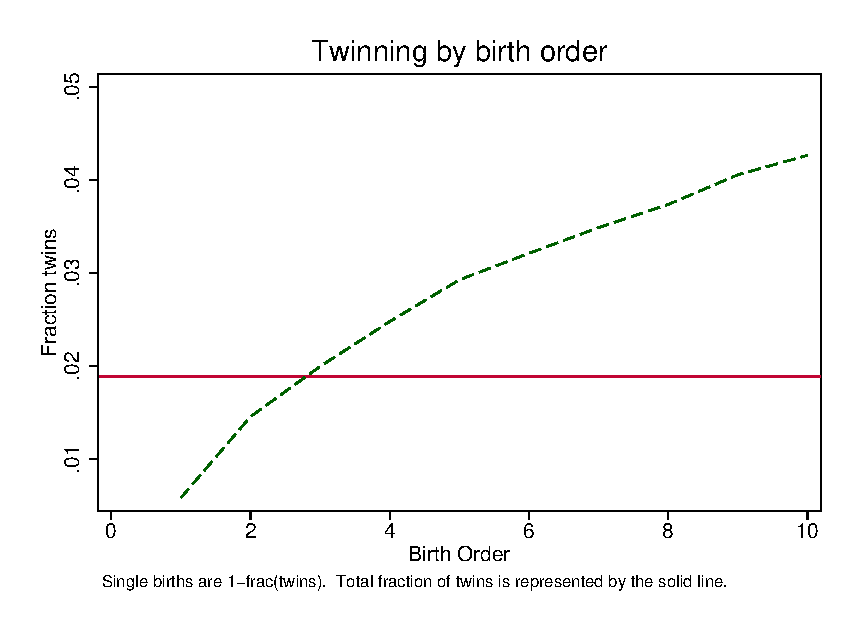
\includegraphics[scale=0.75]{./figures/twinbybord.eps}
\end{figure}
}

\frame{
\begin{figure}[htpb!]
\centering
  \includegraphics[scale=0.75]{./figures/height_country.eps}
  \caption{Height as a Proxy for Health}
  \label{TWINfig:height}
\end{figure}
}


\begin{frame}
\frametitle{Height and Selective Survival}
\begin{figure}[htpb!]
\centering
  \includegraphics[scale=0.75]{./figures/MMRcuts.eps}
\end{figure}
\hyperlink{robust}{\beamergotobutton{Back}}
\end{frame}


\begin{frame}[label=two]
\frametitle{Estimates (2+) Assuming that $\gamma \sim U(0,\delta)$}
\begin{figure}[htpb!]
\centering
  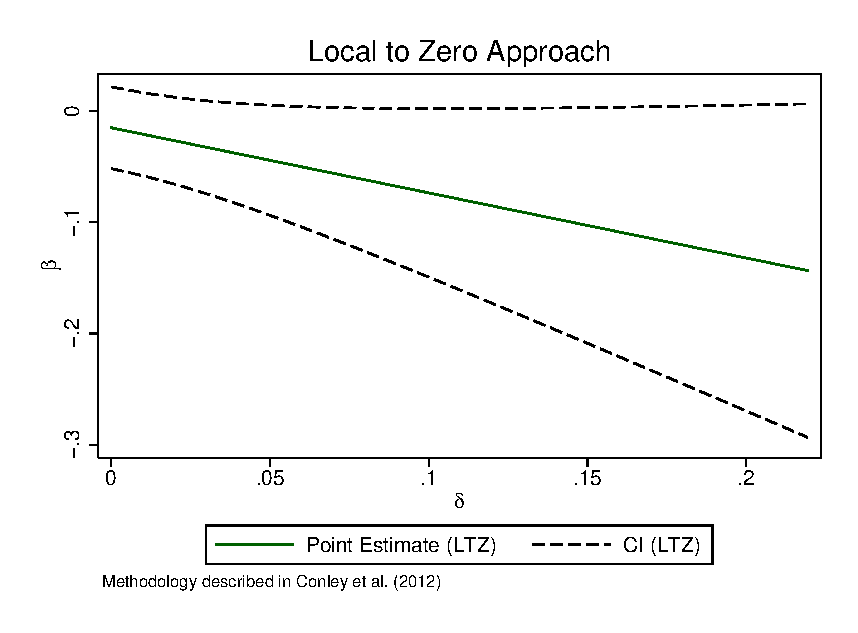
\includegraphics[scale=0.75]{./figures/LTZ_two.eps}
\end{figure}
\hyperlink{Conley}{\beamergotobutton{Back}}
\end{frame}

\begin{frame}[label=four]
\frametitle{Estimates (4+) Assuming that $\gamma \sim U(0,\delta)$}
\begin{figure}[htpb!]
\centering
  \includegraphics[scale=0.75]{./figures/LTZ_four.eps}
\end{figure}
\hyperlink{Conley}{\beamergotobutton{Back}}
\end{frame}

\end{document}

%********************************************************************************
%********************************************************************************
%********************************************************************************
%********************************************************************************
%********************************************************************************
%********************************************************************************
%********************************************************************************
%********************************************************************************
%********************************************************************************
%********************************************************************************
\frame{\frametitle{USA Birth Records}
In preliminary results from National Vital Statistics System (NVSS) which register all births in USA from 1995-2000 (23.5 million observations):
\vspace{5mm}
\begin{itemize}
\item Education is significantly positively related to having a twin
\item Drinking while pregnant is significantly negatively related to having a twin
\item Smoking while pregnant is significantly negatively related to having a twin
\item Age, race and more previous births are significant predictors
\end{itemize}
}
